\section{Experiments}

We now compare the algorithms on their performance solving logistic regression problems. We first outline our experiment methodology, before presenting and discussing our results. Our algorithm implementions and simulations can be found on this \href{https://github.com/EdmundHofflin/Statistical_Machine_Learning_Project}{github repository}.

\subsection{Methodology}

We generate three datasets in the following manner: Given $n$ data points, we sample $\frac{n}{2}$ points from two different $d$ dimensional multivariate normal distributions $\mathcal{N}(\mu_1, \Sigma_1)$ and $\mathcal{N}(\mu_2, \Sigma_2)$. We then add labels $\mathcal{Y} \in \{-1, 1\}$, one for each cluster. For all datasets, we use $d=10$, $n = 1000$, $\mu_1 = \begin{bmatrix} -1 & \ldots & -1 \end{bmatrix}^\top$ and $\mu_2 = \begin{bmatrix} 1 & \ldots & 1 \end{bmatrix}^\top$. In dataset 0, we set the covariace matrices to $\Sigma_1, \Sigma_2 = \mathit{I}_{10}$, whereas in dataset 1 we set $\Sigma_1, \Sigma_2 = 2 \sqrt{10}\mathit{I}_{10}$. In dataset 2, we use non-isotropic covariance matrices given by 
$\Sigma_1 = \begin{bmatrix}
        4\mathit{I}_{5} & \mathbf{0}_{5 \times 5} \\ \mathbf{0}_{5 \times 5} & \mathit{I}_{5}
    \end{bmatrix}$
and $\Sigma_2 = \Sigma_1^{-1}.$
We set the initial iterate to $w_0 = \begin{bmatrix} 0 & \ldots & 0 \end{bmatrix}^\top$.
In SVRG, we set $m = \frac{n}{2}$ so we have $m \in \mathcal{O}(n)$ to guarantee the theoretical convergence rate of SVRG \cite{reddi2016stochastic}. We test all algorithms across the three datasets, while also varying the step-size with $\eta \in \left\{0.05, 0.1, 0.5\right\}$. Finally, our models do not use intercepts.

\subsection{Results}

The results from our simulations are presented in Figure~\ref{fig:sims_results}.
\begin{figure}[h]
    \centering
    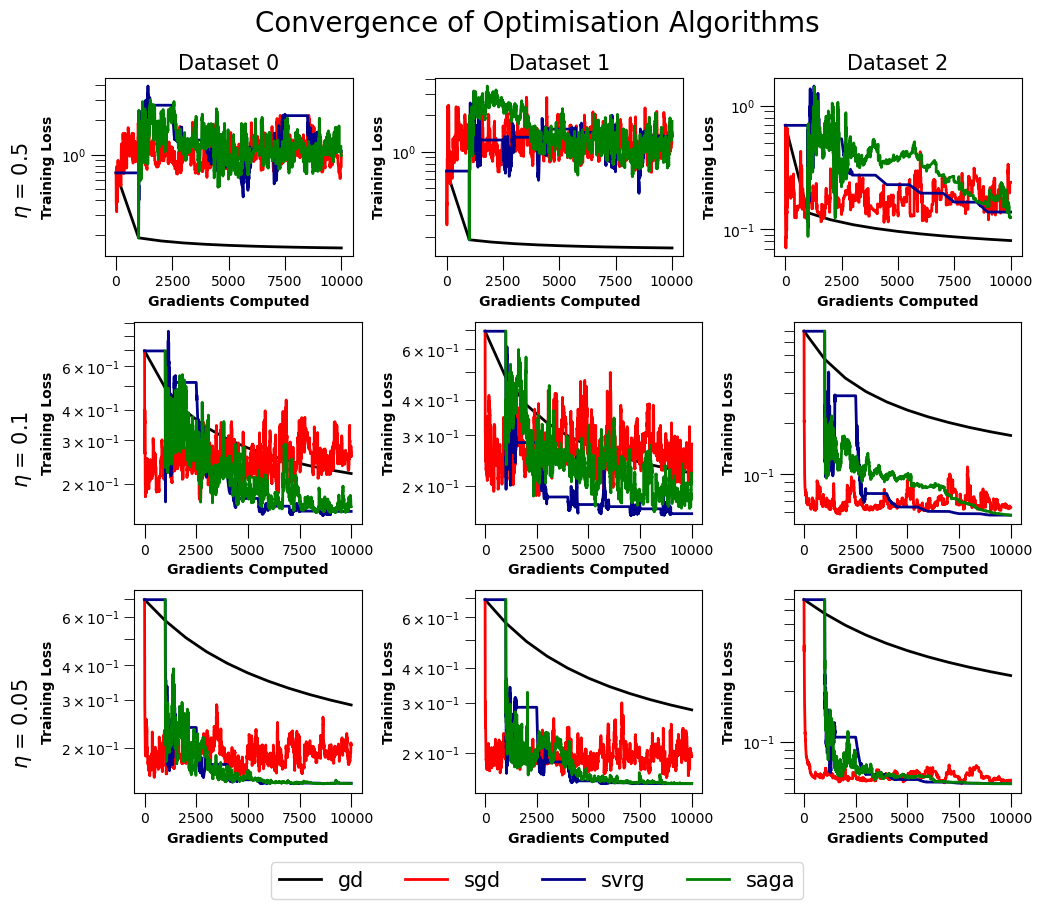
\includegraphics[width=0.85\linewidth]{assets/total_plot.png}
    \caption{Simulation results for datasets $0$, $1$, and $2$, and stepsizes $\eta \in \left\{0.05, 0.1, 0.5\right\}$. In each subplot, we compare the methods with the number of gradients computed on the $x$-axis and the loss in a logarithmic scale on the $y$-axis.}
    \label{fig:sims_results}
\end{figure}
The first major trend is the convergence properties of the four algorithms. GD converges with a rate that is approximately $\mathcal{O}\left(\frac{n}{\epsilon}\right)$. For small step-sizes this is comparatively slow, but it does benefit from always converging to the true solution, regardless of step-size, which is not exhibited by any of the algorithms. Thus, for $\eta = 0.5$, GD is the best performing algorithm. In complete contrast, SGD has a fast rate of convergence given the sample size --- further simulations would be needed to definitely verify that it is indeed $\mathcal{O}\left(\frac{1}{\epsilon^2}\right)$ in real-world computations --- but it is quickly limited by its inability to converge to the true value, instead perpetually bouncing within the neighbourhood around the solution. SVRG and SAGA exhibit the best of both worlds: they descend quickly with the stochastic updates (after their first/initial full gradient computation) and converge towards the true solution. Our simulations do not provide enough evidence to claim that either algorithm is faster than the other, so further experiments are required to verify and compare their respective theoretical rates of convergence, $\mathcal{O}\left(n + \frac{n^{\frac{2}{3}}}{\epsilon}\right)$ and $\mathcal{O}\left(n + \frac{1}{\epsilon}\right)$. Overall, our results exhibit the major theoretical convergence properties of the four algorithms.

The second major trend is the impact of step-sizes. This comes in three forms. Firstly, for sufficiently large step-size, SVRG and SAGA no longer converge. This is evidenced by the simulations with $\eta = 0.5$ for datasets $0$ and $1$, for which neither algorithm successful optimises the problem. This is supported by the theory, which requires particular conditions upon the step-size to guarantee convergence \cite{reddi2016stochastic}. Although not obvious, we believe that SGD does converge: its increases in loss is a consequence of the next impact of step-size. This second impact is that as the step-size increases, the variance of SGD, SVRG, and SAGA also increases. This is entirely expected, as the updates of all three algorithms, and so their variances, are scaled by the step-size. This impact results in SGD's strange convergence with $\eta = 0.5$ for datasets $0$ and $1$: the initial value $\textbf{w}_0$ is a better parameter than most of the parameters in SGD's $\mathcal{O}\left(\eta\right)$ neighbourhood of convergence. The final impact of step-size is the speed of convergence: as the step-size increases, the algorithms initially converge more quickly. This is particularly true for GD and SGD. However, the impact of the step-size on SVRG and SAGA's later convergence behaviour is difficult to gauge from our simulations, so this is an avenue for further exploration.

In addition to the two major trends, we identify two less significant trends. Firstly, as expected,  the variance of the stochastic algorithms increases from dataset $0$ to dataset $1$. This is almost certainly a consequence of the increased variance in those datasets. Secondly, SVRG exhbitis a waterfall-like graph, plateauing at times before resuming a form of stochastic descent. These plateus would correspond to the outer-loop, computing full gradients. 